\section{An exactly solvable serial instance}
\label{sec:instance}

The hypotheses above can all be checked in one model. A scalar spectral
coefficient $a$ and a context coefficient $v$ feed $M$ replicated readouts
$\beta_j$, and the margin is $q=a+bv$ with $b=\sum_j\beta_j$; the loss is
logistic cross-entropy on a training distribution in which spectrum,
context and label coincide, trained by unit-rate gradient flow until the
margin first reaches $m$ (Appendix~\ref{app:math},
Theorem~\ref{thm:astra_serial}).

\begin{theorem}[Serial instance]
\label{thm:instance}
For this model, $\Dcurv(0)=M$ exactly and the residual envelope of
Assumption~\ref{ass:residual} holds with $\mu=(M+1)/4$. For any
$a_0<m$, $v_0\ne0$ and zero-sum readout initialization, the spectral update
at the fitting time satisfies
\[
  0<\frac{a(T_m)-a_0}{m-a_0}\le\frac{1}{1+Mv_0^2},
  \qquad
  0\le q_J(t)-q_F(t)\le\frac{C_0}{p_0Mv_0^2}\ \ (t\le T_m),
\]
where $q_F$ is the margin of the frozen-encoder comparator and
$C_0=1+2(m-a_0)^2/v_0^2$, $p_0=e^{a_0}/(1+e^{a_0})$. Under contextual
reversal at test time the trained model's error tends to $\Phi(m/2\sigma)$
for isotropic Gaussian $(a_0,v_0)\sim\mathcal{N}(0,\sigma^2I)$ while a
spectral-only comparator has zero error, and for $a_0>m/2$ the classifier is
correct at every width. With the readout normalized as $M^{-1/2}Uh$, with
$\mathcal{O}(1)$ entries trained at unit rate, the $M$-dependence
disappears.
\end{theorem}

The mechanism is a replication-induced effective learning rate, made exact
by the layer-balance invariant of gradient flow
\citep{astra_du2018balance}. What is suppressed is the \emph{update} of the
spectral coefficient as a fraction of the fitting task, not the coefficient
itself, which can be informative at initialization and remain so.
Theorem~\ref{thm:twoscale}'s displacement bound is within a factor
$4.5$--$6.3$ of the realised displacement here, and every displayed
quantity agrees with the closed form to
$10^{-11}$ against a full $(2+M)$-parameter integration over $579$ cases
(Appendix~\ref{app:synthetic}). We use a solvable serial CE
example to connect a known optimization-metric imbalance to a finite-margin
encoder-update bound, a joint-versus-frozen trajectory comparison, and an
explicit failure under contextual reversal. Replication changes the
effective learning rate, and its normalization removes the effect. The
example supplies an exact consistency check and a scoped existence result;
it does not establish a new general mechanism of implicit bias.

\begin{figure}[t]
\centering
\IfFileExists{figures/fig1_serial.pdf}{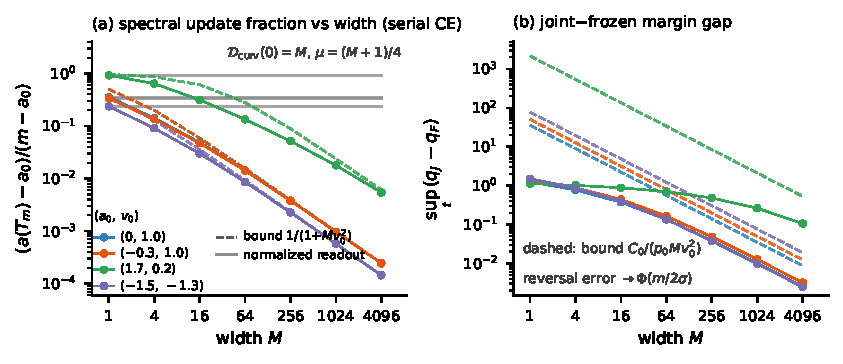
\includegraphics[width=0.92\linewidth]{figures/fig1_serial.pdf}}{\fbox{\rule{0pt}{2.3in}\rule{0.97\linewidth}{0pt}}}
\caption{The serial instance. (a) Spectral update fraction
$(a(T_m)-a_0)/(m-a_0)$ against width $M$ for several $(a_0,v_0)$, with the
exact bound $1/(1+Mv_0^2)$ (dashed) and the normalized-readout control
(flat). (b) Joint-minus-frozen margin gap $\sup_t(q_J-q_F)$ with its bound
$C_0/(p_0Mv_0^2)$. Closed form and full integration agree to $10^{-11}$.}
\label{fig:serial}
\end{figure}
